% Typeset source of the supplement. Generated; the preamble is the paper's.
\documentclass[11pt,a4paper]{article}

% ---------- language and type ----------
\usepackage{polyglossia}
\setdefaultlanguage[variant=british]{english}
\usepackage{fontspec}
\usepackage{unicode-math}
\setmainfont{EBGaramond}[
  Extension = .otf, UprightFont = *-Regular, ItalicFont = *-Italic,
  BoldFont = *-SemiBold, BoldItalicFont = *-SemiBoldItalic,
  Numbers = {Lining,Proportional}, Ligatures = TeX]
\setmonofont{Inconsolatazi4}[Extension = .otf, UprightFont = *-Regular, BoldFont = *-Bold, Scale = MatchLowercase, HyphenChar = None]
\setmathfont{Garamond-Math.otf}[StylisticSet={7,9,10}]
\newfontfamily\titleface{Cormorant Garamond SemiBold}[ItalicFont = {Cormorant Garamond Medium Italic}, Numbers = Lining, Ligatures = TeX]
\newfontfamily\labelface{EBGaramond}[Extension = .otf, UprightFont = *-Medium, Numbers = {Lining,Proportional}]
\newfontfamily\groupface{EBGaramond}[Extension = .otf, UprightFont = *-Medium, ItalicFont = *-MediumItalic, Numbers = {Lining,Proportional}]
\newfontfamily\thmheadface{EBGaramond}[Extension = .otf, UprightFont = *-SemiBold]
\newcommand{\pagelabel}[1]{{\labelface\spacedsc{#1}}}
\newcommand{\spacedsc}[1]{{\scshape\addfontfeatures{LetterSpace=8}\MakeLowercase{#1}}}
\DeclareRobustCommand{\scn}[1]{{\upshape\addfontfeatures{Numbers={Lining,Proportional}}\scalebox{0.84}{#1}}}
\DeclareRobustCommand{\thd}[1]{{\scshape\addfontfeatures{LetterSpace=1.5}\MakeLowercase{#1}}}
\DeclareRobustCommand{\acr}[1]{{\addfontfeatures{Letters=UppercaseSmallCaps,LetterSpace=2}#1}}
\frenchspacing
\displaywidowpenalty=10000

% ---------- body size and leading: 12 on 15.2 ----------
\makeatletter
\renewcommand\normalsize{%
  \@setfontsize\normalsize{12}{15.2}%
  \abovedisplayskip 10\p@ \@plus2\p@ \@minus4\p@
  \abovedisplayshortskip 4\p@ \@plus3\p@
  \belowdisplayshortskip 7\p@ \@plus3\p@ \@minus3\p@
  \belowdisplayskip \abovedisplayskip
  \let\@listi\@listI}
\renewcommand\small{\@setfontsize\small{10.4}{13.4}}
\renewcommand\footnotesize{\@setfontsize\footnotesize{9.4}{12}}
\makeatother
\normalsize

% ---------- page ----------
\usepackage[a4paper,textwidth=132mm,top=33mm,bottom=39mm,headsep=9mm,footskip=14mm,headheight=14pt]{geometry}

\usepackage{amsmath,amsthm}
\usepackage{array}
\usepackage{tabularx}
\newcolumntype{L}[1]{>{\raggedright\arraybackslash}p{#1}}
\newcolumntype{Y}{>{\raggedright\arraybackslash}X}
\usepackage{booktabs}
\usepackage{longtable}
\setlength{\heavyrulewidth}{0.6pt}
\setlength{\lightrulewidth}{0.3pt}
\setlength{\extrarowheight}{2pt}
\usepackage{float}
\usepackage[section]{placeins}
\usepackage{xcolor}
\definecolor{oxford}{RGB}{0,33,71}
\definecolor{oxblood}{RGB}{116,30,44}
\definecolor{racing}{RGB}{24,74,52}
\usepackage{caption}
\DeclareCaptionLabelFormat{sclabel}{{\labelface\scshape\MakeLowercase{#1}}~{\labelface\scn{#2}}}
\captionsetup{figurename=Fig.,labelformat=sclabel,labelsep=period,margin=9mm,font=small,skip=7pt}
\usepackage{enumitem}
\usepackage{etoolbox}

% ---------- headings: centred titling face; italic subheadings and paragraph leads; no bold ----------
\usepackage{titlesec}
\usepackage{titletoc}
\setcounter{tocdepth}{1}
\titlecontents{section}[1.9em]{\small}{\contentslabel{1.9em}}{}{\hfill\contentspage}[\vspace{0.5pt}]
\titleformat{\section}[block]{\centering\titleface\fontsize{17pt}{20pt}\selectfont}{\thesection}{0.7em}{}
\titlespacing*{\section}{0pt}{30pt plus 5pt minus 3pt}{13pt}
\titleformat{\subsection}[block]{\normalsize\itshape}{\upshape\thesubsection}{0.75em}{}
\titlespacing*{\subsection}{0pt}{17pt plus 3pt minus 2pt}{6pt}
\titleformat{\subsubsection}[runin]{\normalsize\itshape}{\upshape\thesubsubsection}{0.6em}{}[.]
\titlespacing*{\subsubsection}{0pt}{9pt plus 2pt minus 1pt}{0.6em}
\titleformat{\paragraph}[runin]{\normalsize\itshape}{}{0pt}{}
\titlespacing*{\paragraph}{0pt}{9pt plus 2pt minus 1pt}{0.6em}

\usepackage{graphicx}
\usepackage{tikz}
\usetikzlibrary{positioning,arrows,calc,shadows}
\usepackage{pgfplots}
\pgfplotsset{compat=1.18}
\usepackage{lettrine}
\setcounter{DefaultLines}{2}
\renewcommand{\LettrineTextFont}{\scshape}
\usepackage{indentfirst}

\widowpenalty=10000
\clubpenalty=10000
\usepackage{needspace}
\setlength{\intextsep}{11pt plus 3pt minus 2pt}
\setlength{\floatsep}{11pt plus 3pt minus 2pt}
\setlength{\textfloatsep}{16pt plus 4pt minus 2pt}
\makeatletter\setlength{\@fptop}{0pt}\setlength{\@fpsep}{18pt plus 4pt}\setlength{\@fpbot}{0pt plus 1fil}\makeatother
\renewcommand{\topfraction}{0.85}\renewcommand{\bottomfraction}{0.7}\renewcommand{\textfraction}{0.12}\renewcommand{\floatpagefraction}{0.75}

% ---------- tables: small, lining tabular figures ----------
\renewcommand{\arraystretch}{1.08}
\AtBeginEnvironment{tabular}{\footnotesize\addfontfeatures{Numbers={Lining,Tabular}}}
\AtBeginEnvironment{tabularx}{\footnotesize\addfontfeatures{Numbers={Lining,Tabular}}}
\AtBeginEnvironment{longtable}{\footnotesize\addfontfeatures{Numbers={Lining,Tabular}}}

\usepackage{microtype}
\usepackage[superscript]{cite}

\makeatletter
\renewcommand\@biblabel[1]{#1.}
\renewenvironment{thebibliography}[1]
  {\section*{\refname}\small
   \list{\@biblabel{\@arabic\c@enumiv}}%
        {\settowidth\labelwidth{\@biblabel{#1}}%
         \leftmargin\labelwidth \advance\leftmargin\labelsep
         \setlength\itemsep{3.5pt plus 1pt}\setlength\parsep{0pt}%
         \usecounter{enumiv}\let\p@enumiv\@empty
         \renewcommand\theenumiv{\@arabic\c@enumiv}}%
   \sloppy\clubpenalty4000\widowpenalty4000\sfcode`\.\@m}
  {\def\@noitemerr{\@latex@warning{Empty `thebibliography' environment}}\endlist}
\makeatother

% ---------- abstract and front-matter notes: centred small-capital label over an inset block ----------
\newenvironment{insetblock}[1]{%
  \begin{center}{\footnotesize\pagelabel{#1}}\end{center}\vspace{-5pt}%
  \fontsize{10pt}{13.4pt}\selectfont
  \begin{list}{}{%
    \setlength{\leftmargin}{9mm}\setlength{\rightmargin}{9mm}%
    \setlength{\listparindent}{0pt}\setlength{\parsep}{6pt plus 2pt minus 1pt}%
    \setlength{\topsep}{0pt}\setlength{\partopsep}{0pt}%
  }\item[]\ignorespaces
}{\end{list}}
\renewenvironment{abstract}{\begin{insetblock}{Abstract}}{\end{insetblock}}

\usepackage{hyperref}
% Forbid mid-URL line breaks (a split URL extracts as a broken reference).
\def\UrlBreakPenalty{10000}
\def\UrlBigBreakPenalty{10000}
\pdfstringdefDisableCommands{\def\acr#1{#1}\def\spacedsc#1{#1}\def\thd#1{#1}\def\scn#1{#1}}
\hypersetup{
  colorlinks=true,
  allcolors=black,
  urlcolor=oxford,
  bookmarksnumbered=true,
  bookmarksopen=true,
  bookmarksopenlevel=1,
  pdfdisplaydoctitle=true,
  pdflang=en-GB,
  pdfauthor={K.R. Ryan},
  pdftitle={Supplement to: The Hidden Microstructure of Shared Balance Concentrated Liquidity},
  pdfsubject={Supplement: simulation tables, tests by scenario, coverage of the formalisation, proofs},
  pdfkeywords={concentrated liquidity, geometric residual, propagation of chaos, interacting particle systems, multi-pool rebalancing, stochastic flow networks, dust ledger, Uniswap V3, Aerodrome, automated market maker, DeFi mechanism design}
}
\urlstyle{same}
\usepackage[bottom]{footmisc}
\renewcommand{\footnotelayout}{\fontsize{8.6pt}{11.4pt}\selectfont}
\setlength{\footnotesep}{9pt}
% Footnotes are marked by symbols, since citations are superscript numerals.
\renewcommand{\thefootnote}{\fnsymbol{footnote}}
\setlength{\skip\footins}{16pt plus 4pt minus 2pt}

% ---------- running head: spaced small capitals, centred; folio at the foot ----------
\usepackage{fancyhdr}
\pagestyle{fancy}
\fancyhf{}
\fancyhead[C]{\footnotesize\spacedsc{The Hidden Microstructure \enspace\textperiodcentered\enspace Supplement}}
\fancyfoot[C]{\small\thepage}
\renewcommand{\headrulewidth}{0pt}
\fancypagestyle{plain}{\fancyhf{}\fancyfoot[C]{\small\thepage}\renewcommand{\headrulewidth}{0pt}}

% ---------- theorems: small-capital label, name in roman, statement in italic ----------
% Each kind of statement keeps its own counter.
\newtheoremstyle{siphon}{11pt plus 2pt minus 1pt}{10pt plus 2pt minus 1pt}{\itshape}{}{}{}{\newline}%
  {{\thmheadface\scshape\MakeLowercase{\thmname{#1}}\thmnumber{ \scn{#2}}}\thmnote{\upshape\enspace\textperiodcentered\enspace #3}\vadjust{\vskip 3pt}}
\theoremstyle{siphon}
\newtheorem{theorem}{Theorem}
\newtheorem{proposition}{Proposition}
\newtheorem{lemma}{Lemma}
\newtheorem{corollary}{Corollary}
\renewcommand\qedsymbol{\raisebox{0.17ex}{\scalebox{0.68}{\ensuremath{\mdlgblksquare}}}}
\providecommand{\proofqed}{%
  \nobreak\hfil\penalty50\hskip2em\hbox{}\nobreak\hfil%
  \hbox{\qedsymbol}%
  {\parfillskip=0pt \finalhyphendemerits=0 \par}}

\usepackage{mdframed}
\newenvironment{codeblock}{%
  \begin{mdframed}[%
    backgroundcolor=white,%
    linewidth=0.5pt,linecolor=black!30,topline=false,bottomline=false,rightline=false,%
    innertopmargin=6pt,%
    innerbottommargin=6pt,%
    innerleftmargin=12pt,%
    innerrightmargin=12pt,%
    leftmargin=1.25em,%
    rightmargin=0pt,%
    skipabove=6pt,%
    skipbelow=6pt%
  ]\footnotesize%
}{%
  \end{mdframed}%
}

\setlength{\parindent}{1.25em}
\setlength{\parskip}{0pt}
\tolerance=1400
\emergencystretch=1.5em

% ---------- the supplement's numbering ----------
\renewcommand{\thetable}{S\arabic{table}}
\renewcommand{\thefigure}{S\arabic{figure}}
\renewcommand{\theequation}{S\arabic{equation}}
\renewcommand{\theproposition}{S\arabic{proposition}}

\begin{document}
\thispagestyle{plain}

\begin{center}
\vspace*{4mm}
{\fontsize{23pt}{28pt}\selectfont\titleface Supplement}\\[10pt]
{\fontsize{14pt}{18.5pt}\selectfont\titleface\itshape The Hidden Microstructure of Shared Balance Concentrated Liquidity:\\
A Master Equation for the Dust Ledger and Propagation of Chaos}\\[15pt]
\rule{16mm}{0.4pt}\\[12pt]
{\fontsize{12pt}{14pt}\selectfont\spacedsc{K.\,R. Ryan}}\\[7pt]
{\fontsize{9pt}{12pt}\selectfont\itshape SSRN 6745218, November 2026 revision}
\end{center}
\vspace{6pt}

\noindent Supplementary tables, figures, equations and statements carry an S prefix. Unprefixed statement, table, figure and equation numbers refer to the paper. The supplement uses the paper's terms and symbols; section numbers also refer to the paper unless a section is identified as part of the supplement.

\vspace{10pt}
\begin{center}
\begin{minipage}{84mm}
\centerline{\footnotesize\pagelabel{Contents}}\vspace{5pt}
\makeatletter\@starttoc{toc}\makeatother
\end{minipage}
\end{center}
\vspace{4pt}

\section{Simulation tables}\label{sup:sim}

These tables provide the simulation detail behind Section~7.1 of the paper. Table~\ref{tab:halfnormal_sim} compares the simulated slack side under the Gaussian law with the half-normal law in the Remark after Proposition~3.

\begin{table}[!htb]
\centering
\caption{The Gaussian case of Proposition~3, $N = 1024$.}
\label{tab:halfnormal_sim}
\begin{tabular}{@{}lrrr@{}}
\toprule
\thd{Quantity} & \thd{Simulated} & \thd{Closed form} & \thd{Ratio}  \\
\midrule
$\mathbb{P}(b = 0)$ & 0.5000 & 0.5000 & 1.0000 \\
$\mathbb{E}[b \mid b > 0]$ & $3.989 \times 10^{-2}$ & $3.989 \times 10^{-2}$ & 1.0000 \\
$\operatorname{Var}(b \mid b > 0)$ & $9.127 \times 10^{-4}$ & $9.085 \times 10^{-4}$ & 1.0047 \\
quantile 0.10 & $6.266 \times 10^{-3}$ & $6.283 \times 10^{-3}$ & 0.9972 \\
quantile 0.25 & $1.590 \times 10^{-2}$ & $1.593 \times 10^{-2}$ & 0.9978 \\
quantile 0.50 & $3.366 \times 10^{-2}$ & $3.372 \times 10^{-2}$ & 0.9982 \\
quantile 0.75 & $5.746 \times 10^{-2}$ & $5.752 \times 10^{-2}$ & 0.9989 \\
quantile 0.90 & $8.225 \times 10^{-2}$ & $8.224 \times 10^{-2}$ & 1.0001 \\
\bottomrule
\end{tabular}
\end{table}

Table~\ref{tab:chaossweep} reports two quantities at each $N$, both multiplied by $N$. The first is the correlation $\rho_N$ between two spokes' balances under the skewed and measured laws. Under the uniform law their balances are uncorrelated, so the table gives the correlation between their squared balances instead. A value in parentheses is below ten Monte Carlo standard errors. The second quantity is a decoupling gap. It measures how much the hub balance a spoke meets depends on that spoke's recent history. Let $G$ be the number of events from other pools since the spoke's previous event, and let $I$ indicate whether its own balance is zero. Both are recorded at the spoke's event. Define
\begin{equation}\label{eq:etaN}
\mathrm{gap}_N  :=  \sum_{g,\,i}\,\mathbb{P}(G = g,\ I = i)\;W_1\bigl(\mathcal{L}(H \mid G = g,\ I = i),\ \mathcal{L}(H)\bigr)
\end{equation}
as the mean distance between the law of the hub balance the spoke meets, given this part of the spoke's history, and its unconditional law. The laws are estimated from histograms; the distance between independent samples from the same law is subtracted to correct for histogram noise.

\begin{table}[!htb]
\centering
\caption{Dependence between spokes and the decoupling gap, each times $N$.}
\label{tab:chaossweep}
\begin{tabular}{@{}rrrrrrr@{}}
\toprule
 & \multicolumn{3}{c}{$N \rho_N$} & \multicolumn{3}{c}{$N\,\mathrm{gap}_N$}  \\
\cmidrule(lr){2-4}\cmidrule(l){5-7}
$N$ & \thd{Skewed} & \thd{Measured} & \thd{Uniform, squares} & \thd{Skewed} & \thd{Measured} & \thd{Uniform}  \\
\midrule
2 & $-0.0201$ & $-0.0063$ & $-0.0031$ & $0.0570$ & $0.0376$ & $0.1141$ \\
4 & $-0.0199$ & $-0.0063$ & $-0.0030$ & $0.0575$ & $0.0379$ & $0.1141$ \\
8 & $-0.0199$ & $-0.0062$ & $-0.0031$ & $0.0577$ & $0.0381$ & $0.1140$ \\
16 & $-0.0198$ & $-0.0062$ & $-0.0032$ & $0.0578$ & $0.0382$ & $0.1139$ \\
32 & $-0.0199$ & $-0.0062$ & $-0.0032$ & $0.0579$ & $0.0382$ & $0.1139$ \\
64 & $-0.0197$ & $-0.0062$ & $-0.0032$ & $0.0579$ & $0.0383$ & $0.1138$ \\
128 & $-0.0198$ & $-0.0064$ & $-0.0032$ & $0.0579$ & $0.0384$ & $0.1137$ \\
256 & $-0.0199$ & $-0.0061$ & $-0.0034$ & $0.0579$ & $0.0382$ & $0.1138$ \\
512 & $-0.0192$ & $-0.0064$ & $-0.0030$ & $0.0577$ & $0.0379$ & $0.1134$ \\
1024 & $-0.0197$ & $-0.0054$ & ($-0.0028$) & $0.0576$ & $0.0381$ & $0.1133$ \\
\bottomrule
\end{tabular}

\vspace{4pt}
\parbox{0.9\linewidth}{\footnotesize Under the Gaussian law the correlation of squared balances times $N$ is about $-9 \times 10^{-5}$, and a longer run at $N = 8$, $16$ and $32$ gives a slope of $-1.00 \pm 0.06$ for the logarithm of the absolute correlation against the logarithm of $N$.}
\end{table}

The gap is of order $1/N$. From $N = 2$ to $1024$, $N\,\mathrm{gap}_N$ is constant to about two per cent and ranges from $0.020$ to $0.114$ across the four laws, in units of $Lw$. Between $95$ and $100\%$ of the gap comes from the case $G = 0$, which has probability $1/N$. In that case the spoke's pool fired at the previous event, so the hub balance it meets is either that event's leftover or zero. Proposition~2 neither uses nor establishes this gap; it is measured on the simulated chain.

Table~\ref{tab:chaoshetero} reports three further runs. Panel~(a) covers unequal spokes. It gives the number satisfying~(12), the largest deviation of their atom from $q$ in Monte Carlo standard errors, and the largest shortfall from $q$ among the other spokes. Panel~(b) covers position size. For $N \geq 16$, it compares the contraction rate of the own-value gap, multiplied by $N$, with $\gamma_+$ and with the rate in Proposition~\ref{prop:sizedrift}(iv), using the simulated ratio of the balance gap to the own-value gap. Panel~(c) covers a common direction. It gives the covariance between two spokes' zero indicators, its limit in $N$ from~(14), and the correlation between their balances at $N = 1024$.

\begin{table}[!htb]
\centering
\caption{Unequal spokes, position size and a common direction.}
\label{tab:chaoshetero}
{\small\itshape (a) Unequal spokes}\par\vspace{3pt}
\begin{tabular}{@{}rrrrrrr@{}}
\toprule
 & \multicolumn{3}{c}{\thd{Skewed}} & \multicolumn{3}{c}{\thd{Measured}}  \\
\cmidrule(lr){2-4}\cmidrule(l){5-7}
$N$ & \thd{spokes} & \thd{largest} $|z|$ & \thd{shortfall} & \thd{spokes} & \thd{largest} $|z|$ & \thd{shortfall}  \\
\midrule
4 & 2 & 0.38 & 0.070 & 1 & 1.52 & 0.044 \\
16 & 4 & 1.37 & 0.036 & 2 & 0.76 & 0.032 \\
64 & 26 & 2.66 & 0.043 & 9 & 3.11 & 0.036 \\
256 & 97 & 3.10 & 0.045 & 15 & 2.28 & 0.036 \\
1024 & 355 & 3.12 & 0.048 & 88 & 2.49 & 0.038 \\
\bottomrule
\end{tabular}

\vspace{1.6ex}
{\small\itshape (b) Position size}\par\vspace{3pt}
\begin{tabular}{@{}lrrr@{}}
\toprule
\thd{Law} & $\gamma_+$ & \thd{simulated} & Proposition~\ref{prop:sizedrift}(iv)  \\
\midrule
Gaussian & 0.0199 & 0.0195--0.0196 & 0.0195 \\
Uniform & 0.1125 & 0.0989--0.0993 & 0.1003 \\
Skewed & 0.1016 & 0.0992--0.0999 & 0.0995 \\
Measured & 0.0795 & 0.0781--0.0786 & 0.0785 \\
\bottomrule
\end{tabular}

\vspace{1.6ex}
{\small\itshape (c) A common direction}\par\vspace{3pt}
\begin{tabular}{@{}rrrrrr@{}}
\toprule
 & & \multicolumn{3}{c}{\thd{covariance of zero indicators}} &  \\
\cmidrule(lr){3-5}
$\tau_{\mathrm{r}}$ & $r$ & \thd{limit} & $N = 16$ & $N = 1024$ & $\rho_{1024}$  \\
\midrule
1 & 0.3 & 0.00144 & 0.00131 & 0.00143 & 0.0061 \\
1 & 0.6 & 0.00574 & 0.00524 & 0.00573 & 0.0250 \\
1 & 0.9 & 0.01292 & 0.01180 & 0.01290 & 0.0583 \\
10 & 0.3 & 0.00359 & 0.00358 & 0.00359 & 0.0151 \\
10 & 0.6 & 0.01436 & 0.01433 & 0.01435 & 0.0623 \\
10 & 0.9 & 0.03230 & 0.03224 & 0.03229 & 0.1471 \\
\bottomrule
\end{tabular}
\end{table}



\section{The steps of the leftover by portfolio}\label{sup:steps}

Table~\ref{tab:ladder_portfolio} breaks the first column of Table~8 down by portfolio. It gives the share of swap-corrected range changes on which each step names the token that holds the leftover, beside the share that a guess from each pool's mix of leftover tokens reaches.

\begin{table}[!htb]
\centering
\caption{Right token on swap-corrected range changes, by portfolio and step (\%).}
\label{tab:ladder_portfolio}
\begin{tabular}{@{}lrrrrrr@{}}
\toprule
 & & \multicolumn{4}{c}{\thd{Step}} &  \\
\cmidrule(lr){3-6}
\thd{Portfolio} & \thd{Events} & \thd{(i)} & \thd{(ii)} & \thd{(iii)} & \thd{(iv)} & \thd{Pool mix}  \\
\midrule
A & 12{,}515 & 15.5 & 13.4 & 61.3 & 100.0 & 61.5 \\
B & 13{,}764 & 37.8 & 38.2 & 84.6 & 100.0 & 85.4 \\
C & 3{,}862 & 20.1 & 20.0 & 63.4 & 100.0 & 62.5 \\
D & 807 & 8.2 & 7.7 & 28.0 & 100.0 & 51.3 \\
E & 2{,}241 & 41.4 & 42.4 & 87.2 & 100.0 & 86.8 \\
F & 4{,}024 & 24.9 & 24.9 & 73.8 & 100.0 & 73.9 \\
G & 2{,}372 & 16.3 & 15.5 & 50.3 & 100.0 & 58.9 \\
H & 1{,}626 & 5.0 & 2.6 & 36.0 & 100.0 & 53.0 \\
I & 680 & 10.3 & 8.4 & 20.1 & 100.0 & 49.9 \\
J & 269 & 8.6 & 7.8 & 36.1 & 100.0 & 48.4 \\
Other depositors & 26{,}620 & 31.1 & 30.9 & 77.4 & 100.0 & 78.4 \\
\midrule
Total & 68{,}780 & 27.3 & 26.8 & 72.0 & 100.0 & 73.9 \\
\bottomrule
\end{tabular}
\end{table}

Figure~\ref{fig:perevent_scatter} sets the leftover predicted at step~(iii), from the pre-swap price with the swap's amounts, against the leftover on chain for the swap-corrected range changes, both as fractions of the withdrawn value.

\begin{figure}[!htb]
\centering
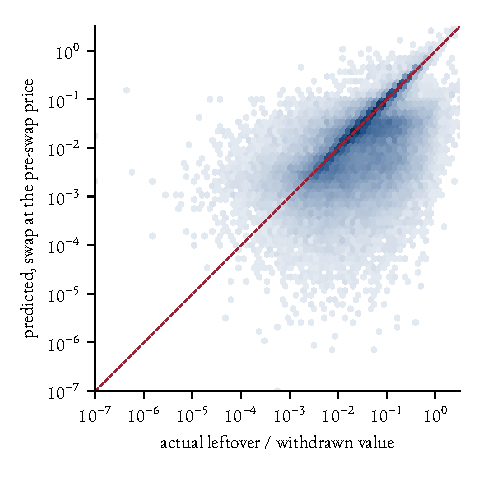
\includegraphics[width=0.46\textwidth]{figures/fig_ladder_rung3.pdf}
\caption{Step~(iii) against the chain. Shading is by the square root of the number of events in a bin, and the dashed line is equality. Three values below $10^{-7}$ are drawn at that level.}
\label{fig:perevent_scatter}
\end{figure}


\section{Auxiliary indexers}\label{sup:indexers}

Two auxiliary indexers support the validation. An admin-operation indexer scans \acr{PM}~V9 transactions to block 44{,}277{,}369. It finds no administrative call that changes the ledger outside the events used in the paper. The only decoded administrative operations, $27$ in number, are deposits already recorded as \texttt{DustCredited} events.

A second indexer filters Pool.Swap events by the indexed sender topic. It records 73{,}350 swaps issued by \acr{PM}~V9 across its 52 managed pools to block 45{,}746{,}143, one for each rebalance that swapped. These events provide the swap-correction inputs $(\sigma_x, \sigma_y)$. In that window, swaps occur on 96\% of range-changing rebalances and 58\% of all rebalances.


\section{The Foundry suite, scenario by scenario}\label{sup:foundry}

Appendix~H of the paper maps the tests to the statements. This section describes each group of tests and gives the figures captured.

\subsection{Reproduction}

The network-free tests run locally:

\begin{codeblock}\begin{verbatim}
forge test -vv --no-match-contract Fork
\end{verbatim}\end{codeblock}

The full suite, including the twelve fork tests, runs with:

\begin{codeblock}\begin{verbatim}
RPC_BASE_ALCHEMY=https://mainnet.base.org forge test -vv
\end{verbatim}\end{codeblock}

Recorded \texttt{forge test -vv} output is provided in \texttt{foundry/PROOF\_OUTPUT.md} and serves as the regression target. It also records which tests fail under each of twelve deliberate faults in the model, the reference contracts and the tested formulas.

\subsection{Theorem~1 on the integer pool model}

\texttt{MasterEquationT1Mock} tests the anchor case from the prior paper (\acr{SSRN} 6686798) in the integer model. The position is withdrawn after a 200-tick price move and minted into a wider range. For each mint inside the new range, three checks compare the result with Theorem~1 without reusing the model's liquidity formula. One additional liquidity unit would require more of at least one token than was offered. The binding token is used up to within the amount consumed by one liquidity unit. The leftover of the other token equals the amount offered less the binding amount multiplied by $g_y/g_x$ or its reciprocal.

The tests cover an empty ledger, a standing balance in either token, swaps both short of and beyond the amount that would leave nothing, a price outside the new range, and a leftover drawn into another position's mint. In the empty-ledger case, the leftover is within 5\% of the residual reported for this case in the prior paper. Outside the new range, the mint is single-sided and the other token is credited in full. An eighth test compares the mock pool shared with the prior paper's suite with the model.

\subsection{Proposition~1 and its corollaries on the integer pool model}

\texttt{MasterEquationP1Mock} checks each statement with its own formula. The amounts make integer rounding less than one part in $10^{12}$; the tolerance is one part in $10^{9}$ of the value involved. The proposition is checked in share form on 400 mints at arbitrary prices, ranges and inputs. Of these, 178 leave $T_a$ and 222 leave $T_b$.

Corollary~1(i) is checked at 13 displacements, spanning beyond both bounds of the old range, and at three widths of the new range. The leftover follows the direction of the move and is worth $\alpha(\ell)\,V$. For Corollary~1(ii), a standing balance worth nine tenths of $\alpha(\ell)\,V$, in three compositions, leaves the token unchanged; a balance of $\alpha(\ell)\,V$ held in the token used up in part~(i) leaves no leftover; eleven tenths of it shifts the leftover to that token. Corollary~2 is checked at five displacements and with residuals of zero, 4\% and 50\% in either direction. The final displacement and 4\% residual are the example in Section~4.1 of the paper.

\subsection{Theorem~1 against two position managers}

\texttt{MasterEquationT1Fork} and \texttt{MasterEquationT1ForkUniV3} run the same four scenarios against the Aerodrome Slipstream\footnote{\texttt{0x827922686190790b37229fd06084350E74485b72} on Base.} and Uniswap V3\footnote{\texttt{0x03a520b32C04BF3bEEf7BEb72E919cf822Ed34f1} on Base.} position managers, in the \acr{WETH}/\acr{USDC} pools of tick spacing 100 and of fee 500. Table~\ref{tab:foundry-forks} gives the ledger entries left. The entries returned by each transaction match Theorem~1's predictions, as does the minted liquidity. For the no-swap case, the predictions were stated before the transaction.

\begin{table}[!htb]
\centering
\caption{Ledger entries left, predicted and returned, on two position managers.}
\label{tab:foundry-forks}
\begin{tabular}{@{}llrr@{}}
\toprule
\thd{Scenario} & \thd{Entry} & \thd{Slipstream} & \thd{Uniswap V}\scn{3}  \\
\midrule
No swap                      & \acr{WETH} (wei) & 706 & 213 \\
                             & \acr{USDC} (raw) & 249{,}980{,}633 & 418{,}199{,}469 \\
With a swap                  & \acr{WETH} (wei) & 283 & 941 \\
                             & \acr{USDC} (raw) & 363{,}150{,}183 & 612{,}788{,}020 \\
Three in a row, first        & \acr{WETH} (wei) & 69 & 292 \\
                             & \acr{USDC} (raw) & 142{,}456{,}347 & 405{,}158{,}378 \\
Three in a row, second       & \acr{WETH} (wei) & 594 & 368 \\
                             & \acr{USDC} (raw) & 58{,}204{,}098 & 395{,}322{,}046 \\
Three in a row, third        & \acr{WETH} (wei) & 704 & 211 \\
                             & \acr{USDC} (raw) & 249{,}980{,}631 & 418{,}199{,}467 \\
Cross-pool, before the mint  & \acr{WETH} & 0.706160093942592145 & 0.605533377748812294 \\
Cross-pool, after the mint   & \acr{WETH} & 0.484375590415751947 & 0.000000000000001723 \\
\bottomrule
\end{tabular}
\end{table}

In the swap scenario, the manager sells 0.05 \acr{WETH} in the pool between withdrawal and mint. The prediction uses the withdrawn amounts, the standing balance, and the swap legs and post-swap price from the pool's \texttt{Swap} event.

In the cross-pool scenario, the first position moves to a range that needs less \acr{WETH} than it holds. A second position is then opened with only its other token in a pool that shares \acr{WETH} with the first (\acr{WETH}/\acr{AERO} on Slipstream or \acr{WETH}/cbBTC on Uniswap V3). The second mint draws its \acr{WETH} from the ledger; the resulting entry is shown in the table's last row.

\subsection{Proposition~1 against two position managers}

\texttt{MasterEquationP1Fork} and \texttt{MasterEquationP1ForkUniV3} start with an empty ledger and a position whose range lies 300 ticks below the price. Without a swap, the position would leave \acr{USDC}. From this starting state, each manager is tested with swaps equal to nine tenths and eleven tenths of the amount that would leave nothing, calculated without fee or price impact (Table~\ref{tab:foundry-sign}).

\begin{table}[!htb]
\centering
\caption{The token left by a swap short of and beyond the exact amount, in \acr{USDC}.}
\label{tab:foundry-sign}
\begin{tabular}{@{}llrr@{}}
\toprule
\thd{Swap} & \thd{Quantity} & \thd{Slipstream} & \thd{Uniswap V}\scn{3}  \\
\midrule
One tenth short  & \acr{USDC} left                      & 206.69 & 188.97 \\
                 & Proposition~1 & 206.31 & 189.10 \\
One tenth beyond & value of the \acr{WETH} left         & 179.61 & 185.83 \\
                 & Proposition~1 & 180.01 & 185.68 \\
\bottomrule
\end{tabular}
\end{table}

The swap that falls short leaves \acr{USDC}, the token the position held, and uses up the \acr{WETH} to within a few hundred wei. The swap that goes beyond leaves \acr{WETH}, the token it bought, and no \acr{USDC}. The rows labelled Proposition~1 give the predicted leftover value. It is the swap's shortfall or excess divided by the share of the token used up that the new range requires. This is the proposition's expression when the swap is taken at the pool price. The measured values differ by less than $0.3\%$, reflecting the pool fee and swap price impact.

\subsection{Theorem~2 against two position managers}

\texttt{MasterEquationT2Fork} and \texttt{MasterEquationT2ForkUniV3} hold two positions in pools that share \acr{WETH}. The tests rebalance them alternately, eight times, without a swap, into ranges of different widths and offsets. For each token, the test adds the amount each position would return at its pool's price to the ledger entry. This gives the total $M_i$ in~(6).

On both exchanges, no rebalance increased a total. Each rebalance reduced the total of a token in its own pool by at most one base unit; totals for tokens outside that pool did not change. Over the run, the \acr{WETH} total fell by 8 wei, one at each rebalance. Each other total fell by 4 base units, one at each rebalance of its pool. These units are the rounding remainders kept by the pool when it rounds a mint up. After every call, the ledger equalled the tokens held by the contract.

Theorem~2 has no network-free test. Without token custody, a network-free test could verify only its own bookkeeping. The transfers between positions of Lemma~1 are computed on the V9 record in Section~8.3 and are not Foundry-tested.


\section{Coverage of the Lean formalisation}\label{sup:lean}

The exact statements and the event-by-event part of the model are also formalised in Lean~4 against mathlib. A formalisation is a machine-checked proof of a mathematical statement. It does not check contract code; that is the task of the Foundry suite. The formalisation uses real arithmetic, so it does not cover the pool's integer rounding. Table~\ref{tab:lean} gives the coverage statement by statement.

For the model of Section~6, the formalisation covers the kernel and its single-event consequences. It does not cover the statements about laws, which rely on the proofs in Appendix~F of the paper and Section~\ref{sup:proofs} of this supplement.

\begin{table}[!htb]
\centering
\caption{The Lean formalisation, statement by statement.}
\label{tab:lean}
\begin{tabular}{@{}>{\raggedright\arraybackslash}p{\dimexpr0.30\linewidth-1.33\tabcolsep\relax}>{\raggedright\arraybackslash}p{\dimexpr0.38\linewidth-1.33\tabcolsep\relax}>{\raggedright\arraybackslash}p{\dimexpr0.32\linewidth-1.33\tabcolsep\relax}@{}}
\toprule
\thd{Statement} & \thd{Machine-checked} & \thd{Not formalised}  \\
\midrule
Theorem~1 & in full, with the mint as a linear programme & integer rounding \\
\addlinespace[2pt]
Proposition~1, Corollaries~1 and~2 & in full & -- \\
\addlinespace[2pt]
Theorem~2 & in full & integer rounding \\
\addlinespace[2pt]
Lemma~1 & parts (i) to (iv), under the mint's budget & -- \\
\addlinespace[2pt]
Kernel~(8) & derived from Theorem~1 on the leading-order inputs & the remainder of order $w$ \\
\addlinespace[2pt]
Lemma~2 & identity~(25), invariant set, contraction under one event & the stationary law, its uniqueness and convergence \\
\addlinespace[2pt]
Proposition~2 & the first step, one entry to one entry & the bound, the fixed point, the covariances \\
\addlinespace[2pt]
Proposition~3 & the side identity, the value of $q$, the slack-side distance at one event & the passage to the stationary law \\
\addlinespace[2pt]
Gaussian case of Proposition~3 & $q = 1/2$ and the half-normal mean & the conditioning to $[-K, K]$ \\
\addlinespace[2pt]
Propositions~4 and~5, Lemma~3 & -- & all \\
\addlinespace[2pt]
Proposition~\ref{prop:sizedrift} & parts (i) and (iii); (ii) and (iv) given the conditional means & the expectation in (iv) \\
\bottomrule
\end{tabular}
\end{table}

Some rows of the table need more than a cell holds. In Theorem~1 the mint is stated as a linear programme whose optimum is~(3), so that the programme is part of what is proved and not a premise. In Proposition~1 and its corollaries $\alpha(\ell)$ is defined algebraically in the prices and identified with the expression of Section~5.1. Inside the old range Corollary~1(ii) and Corollary~2 are stated in $\alpha(\ell)$, and at or beyond a bound in the surplus of the swap-free mint, which is then the whole withdrawn value. The condition on Lemma~1 is that a mint cannot take more than the position's own withdrawal and the whole of the ledger. The kernel~(8) is obtained from Theorem~1 applied to the inputs the swap leaves, and is not posited. For Lemma~2 the positivity of the imbalance on the invariant set is checked with the three steps listed. The identity behind the atom of Proposition~3 is that after an event of its own pool a spoke's entry is zero exactly when $\eta \varepsilon \geq 0$. It is checked for every state with a positive imbalance, and the slack-side distance is that of the leftover from $c_0 Lw\,|\varepsilon|$. The first step of the proof of Proposition~2 is that, under the affine form the kernel takes on a positive imbalance, a change made to one entry of the ledger is, after any finite sequence of events, a change in at most one entry.


\section{The first set of replays}\label{sup:replays}

The paper compares the model with the chain record using two sets of replays (Section~8.4). This section gives the first set in full. Each step shuffles another feature of the events within each pool and portfolio, while retaining the earlier shuffles. The paper uses these results only to identify which steps include the chain value and which exclude it.

For each pair, the statistic is the covariance between its two zero indicators, divided by the standard deviation of that covariance under a time shift of one entry's sequence. Table~\ref{tab:ladder_v9} gives the mean at each step for the 59 pairs that are never in one pool and, separately, for the 39 of them that share a partner token. It also gives the standard deviation of the 59-pair mean across replays and, as in Table~12, the number of pairs dependent beyond the time-shift null. The final row draws every outcome independently. Its standard deviation, $0.13$, is the scale used to judge the chain value.

\begin{table}[!htb]
\centering
\caption{Mean standardised covariance of zero indicators on chain and in replays of the record.}
\label{tab:ladder_v9}
\begin{tabular}{@{}lrrrr@{}}
\toprule
 & \multicolumn{2}{c}{\scn{59}\thd{ pairs}} & \thd{Sharing} & \thd{Dependent}  \\
\thd{Shuffled} & \thd{Mean} & \thd{Replay s.d.} & \thd{a partner} & \thd{pairs}  \\
\midrule
Nothing (chain)                                & 0.47 &      & 0.75 & 14 \\
1.\ Residual, by direction and mismatch size    & 0.43 & 0.08 & 0.66 & 11 \\
2.\ Residual, by direction                      & 0.42 & 0.09 & 0.67 & 11 \\
3.\ Direction and residual                      & 0.29 & 0.12 & 0.40 & 8 \\
4.\ Same-range outcomes, by week                & 0.05 & 0.12 & 0.08 & 5 \\
5.\ Same-range outcomes                         & 0.02 & 0.12 & 0.03 & 4 \\
6.\ Order of events                             & 0.00 & 0.06 & 0.00 & 2 \\
\midrule
Independent outcomes                           & 0.00 & 0.13 & 0.00 & 3 \\
\bottomrule
\end{tabular}
\end{table}

The residuals shuffled are those of the range changes whose residual is measured, with the direction that of the corrective swap, and a class of mismatch at step~1 is a fifth of a pool's events in one direction, ranked by the size of the position's own mismatch. With the direction read as the side of the old range's centre on which the event fires, the row of the residual by direction reads $0.37$ for the 59 pairs and $0.61$ for the 39. At step~4 the events not yet shuffled are the same-range rebalances together with the range changes whose residual was not measured, and shuffling the same-range ones alone gives values within $0.01$ of those in the table.

At a shuffled event the side of the leftover follows the sign of $\eta\varepsilon$ in the token's frame, so the standing balance never decides it. The two last events of a pair never in one pool lie in different pools and are shuffled separately, so by Lemma~3 the mean of the indicator covariance at each step is known exactly from the record. The replays reproduce it at every step, which checks the replays and not the chain.

A same-range rebalance usually repeats its pool's last outcome. Retaining same-range outcomes therefore also preserves the range-change outcomes. The reduction at each step cannot be read as a separate share of causation. The breakdown by residual, direction and timing that the figures suggest is withdrawn. The figures are given for the record, in the order of the shuffles. Shuffling the residual within pool and direction lowers the chain value by about a tenth, nearly all at the first step. Shuffling direction within each pool lowers it by a further fifth to three tenths. The larger reduction uses direction from the swap; the smaller uses which side of the old range's centre the event falls on.

Shuffling same-range outcomes lowers the value by more than half, most of that when the shuffle is confined to a calendar week. The reduction is as large when they are shuffled within their direction instead. Shuffling event order lowers it by the remaining thirtieth. Pairs whose tokens share no partner show no dependence on average at any step, although two of the twenty are dependent on chain and remain so.

The figures are exact for the record, but the chain value is only about four null standard deviations from zero. Each estimate is therefore uncertain by about a quarter of that value. The steps that shuffle same-range outcomes were added after the first results had been seen. Only those steps are resolved. The chain value lies inside the central $95\%$ of replays at every step that retains same-range outcomes; no replay reaches it at a step that shuffles them. The data locate the excess of positive dependence in same-range rebalances but do not divide it between residual and direction.


\section{Proofs for the extensions of the model}\label{sup:proofs}

The paper states Propositions~4 and~5 and Lemma~3 in Section~6.2 and proves them here. The two propositions are proved as the changes they make to the proof of Proposition~2 in Appendix~F, whose equations and configurations (Table~17) they use. The last subsection states and proves the result on position size that Section~6.3 describes.

\subsection{Unequal spokes}

\begin{proof}[Proof of Proposition~4]
Only the changes to the proof of Proposition~2 are given here. At an event of pool $k$ let
\[
\zeta := c_0 \eta \varepsilon \in [-\kappa_k, \kappa_k], \qquad A_\eta = L_k w_k + \eta\,(B_k - H) .
\]

\emph{Invariant set.} On $[0, b^*]^{N+1}$ the imbalance satisfies $L_k w_k - b^* \leq A_\eta \leq L_k w_k + b^*$, so a leftover is at most $\kappa_k\,(L_k w_k + b^*)$, which is at most $b^*$ by the definition of $b^*$ in~(10), and $A_\eta > 0$ by the inequality there. The set is invariant, and on it the kernel of every pool reads
\[
H' = \zeta^+ A_\eta, \qquad B_k' = \zeta^- A_\eta .
\]
The condition is sufficient and cannot be dropped. If $b^*$ exceeds the smallest size and the residual laws charge their extremes in both directions, events of the pool that attains the maximum can carry the hub balance towards $b^*$, and a smaller pool with an empty balance then has $A_+ < 0$. With one bound $\kappa$ for all pools the condition says that the largest position is less than $(1 - \kappa)/\kappa$ times the smallest.

\emph{Stationary law and fixed point.} The identity~(25) holds for each pool with its own residual. With $\kappa_1^* := \max_k c_0\,\mathbb{E}|\varepsilon|$, two copies under one driving sequence satisfy
\[
\mathbb{E}\bigl[\|X_1' - X_2'\|_1 \mid X_1, X_2\bigr]  \leq  \bigl(1 - (1 - \kappa_1^*)\min_k \varpi_k\bigr)\,\|X_1 - X_2\|_1 ,
\]
which gives the unique stationary law as in Lemma~2. With $\pi_H^{(k)}$ and $\mu_k'$ as in the fixed-point system~(11), the laws of $H'$ and $B_k'$ after an event of pool $k$ from $(H, B_k) \sim \pi_H \otimes \mu_k$, let $\Gamma_k$ be their joint law. By~(25) and the convexity of $W_1$ under mixtures, the map defined by the right sides of~(11) contracts $W_1(\pi_{H,1}, \pi_{H,2}) + \sum_k \varpi_k\,W_1(\mu_{k,1}, \mu_{k,2})$ by the factor $\kappa_1^*$, so the solution exists and is unique.

\emph{One register.} The one-register argument is unchanged. The size of a pool enters the imbalance of two states equally and cancels in their difference.

\emph{A defect of second order.} Let $\bar\pi^N := \pi_H \otimes \mu_1 \otimes \cdots \otimes \mu_N$. After an event of pool $k$ from $\bar\pi^N$ the pair $(H, B_k)$ has law $\Gamma_k$, with marginals $\pi_H^{(k)}$ and $\mu_k$. Here $\pi_H^{(k)}$ is not $\pi_H$, so one event of a given pool does move the law of the hub balance, which is a change of first order. Averaged over the firing pool it does not, by the second part of~(11). With $(a_k, c_k)$ and $(a_k', c_k')$ independent with law $\Gamma_k$, and $x[a, c]$ the state with hub balance $a$, balance $c$ on spoke $k$ and the other balances drawn from their $\mu_j$, the states $x[a_k, c_k']$ and $x[a_k', c_k]$ have law $\pi_H^{(k)} \otimes \bigotimes_j \mu_j$, and the mixture of these laws over $k$ is $\bar\pi^N$. Hence, for the chain started from $X_0 \sim \bar\pi^N$,
\[
\mathbb{E}\,g(X_1) - \mathbb{E}\,g(X_0)  =  \sum_k \frac{\varpi_k}{2}\,\mathbb{E}\bigl[\,g(x[a_k, c_k]) + g(x[a_k', c_k']) - g(x[a_k, c_k']) - g(x[a_k', c_k])\,\bigr] ,
\]
which is~(29) with the firing pool drawn with probabilities $\varpi_k$. The bound that follows~(29) applies to each term.

\emph{The two-perturbation sum.} Let the observed registers be the hub and the spokes in $T$, and define $\mathcal{S}_T$ as in~(30) with the second perturbation started from a spoke drawn with probabilities $\varpi_k$. Without symmetry between the pools the configurations of the two perturbations are written
\[
\begin{array}{@{}ll@{}}
{[0]} & \text{together on the hub,} \\
{[j]} & \text{together on spoke } j, \\
{(0, j)} & \text{apart, on the hub and spoke } j, \\
{(i, j)} & \text{apart, on spokes } i \neq j .
\end{array}
\]
For pool $k$ let
\[
\gamma^k_\pm := \mathbb{E}[\zeta^\pm], \qquad \varsigma^k_\pm := \mathbb{E}[(\zeta^\pm)^{1/2}], \qquad \varsigma^k := \varsigma^k_+ + \varsigma^k_- \leq \varsigma^* .
\]
Then
\begin{align*}
(\mathcal{Q}\varphi)[0] &= \textstyle\sum_k \varpi_k\bigl(\gamma^k_+\,\varphi[0] + \gamma^k_-\,\varphi[k]\bigr), \\
(\mathcal{Q}\varphi)[j] &= (1 - \varpi_j)\,\varphi[j] + \varpi_j\bigl(\gamma^j_+\,\varphi[0] + \gamma^j_-\,\varphi[j]\bigr), \\
(\mathcal{Q}\varphi)(0, j) &= \varpi_j\bigl(\gamma^j_+\,\varphi[0] + \gamma^j_-\,\varphi[j]\bigr) + \textstyle\sum_{k \neq j} \varpi_k\bigl(\varsigma^k_+\,\varphi(0, j) + \varsigma^k_-\,\varphi(k, j)\bigr), \\
(\mathcal{Q}\varphi)(i, j) &= (1 - \varpi_i - \varpi_j)\,\varphi(i, j) + \varpi_i\bigl(\varsigma^i_+\,\varphi(0, j) + \varsigma^i_-\,\varphi(i, j)\bigr) \\
&\qquad + \varpi_j\bigl(\varsigma^j_+\,\varphi(0, i) + \varsigma^j_-\,\varphi(i, j)\bigr).
\end{align*}
Let
\begin{align*}
\Lambda &:= \frac{1}{1 - \kappa_1^*}\Bigl(1 + \sum_{k \in T} \frac{\gamma^k_-}{1 - \gamma^k_-}\Bigr), \\
d_{ij} &:= \varpi_i\,(1 - \varsigma^i_-) + \varpi_j\,(1 - \varsigma^j_-), \\
\Lambda_1 &:= \frac{1}{1 - \varsigma^*}\Bigl(\max_{j \in T}\Bigl[\frac{1}{1 - \gamma^j_-} + \sum_{k \in T,\,k \neq j} \frac{\varpi_k\,\varsigma^k_-}{d_{kj}}\Bigr] + \varpi^*\,\kappa_1^*\,\Lambda\Bigr), \\
\Lambda_0 &:= \frac{1}{1 - \varsigma^*}\Bigl(\varpi^*\,\kappa_1^*\,\Lambda + \Lambda_1 \sum_{k \in T} \varpi_k\,\varsigma^k_-\Bigr).
\end{align*}
A function with $\varphi \geq \mathbf{1}_{\symup{obs}} + \mathcal{Q}\varphi$ is then given, for two perturbations together, by
\[
\varphi[0] = \Lambda, \qquad
\varphi[j] = \begin{cases} \Lambda + \dfrac{1}{\varpi_j\,(1 - \gamma^j_-)} & \text{for } j \in T, \\[1.6ex] \Lambda & \text{for } j \notin T, \end{cases}
\]
and, for two perturbations apart, by
\[
\varphi = \begin{cases} \Lambda_1 + 1/d_{ij} & \text{if both are on spokes of } T, \text{ on } i \text{ and } j, \\ \Lambda_1 & \text{if one is on a spoke of } T, \\ \min(\Lambda_0, \Lambda_1) & \text{if neither is.} \end{cases}
\]
The inequality is checked configuration by configuration as in the equal case, the hub's own rows $[0]$, $(0, j)$ with $j \in T$ and $(0, j)$ with $j \notin T$ holding by the choices of $\Lambda$, $\Lambda_1$ and $\Lambda_0$. Therefore
\[
\mathcal{S}_T  \leq  \varpi_T\,\Lambda_1 + \Lambda_0  \leq  \frac{m\,(\varpi^* + 2 \varpi_T)}{(1 - \varsigma^*)^4} ,
\]
using $\Lambda \leq m/(1 - \varsigma^*)^2$ and $\Lambda_1 \leq 2m/(1 - \varsigma^*)^3$, and the distance in the statement is at most $b^*\,\mathcal{S}_T$ by the telescoping of the proof of Proposition~2.

\emph{Each spoke, and the means.} After an event of pool $k$ the balance of spoke $k$ is $\zeta^- A_\eta$ with $A_\eta > 0$ and $|A_\eta - L_k w_k| \leq b^*$, and the mark is independent of the state. The proof of Proposition~3 applies to pool $k$ with its own size and residual law, under $\pi^N$ and under the fixed point alike. The kernel is affine with coefficients independent of the state, so the means under $\pi^N$ satisfy a linear system with a unique solution, and the means of $\pi_H$ and the $\mu_k$ satisfy the same system by~(11).
\end{proof}

Three limits of the statement should be kept in view. It is an upper bound in units of $b^*$, which is set by the pool with the largest $\kappa_k L_k w_k/(1 - \kappa_k)$, so for a spoke much smaller than that pool it is informative only when $\varpi^*$ is correspondingly small, and the relative error $b^*/(L_k w_k)$ in the scale of $\rho_{+,k}$ is below one but need not be small. The closed form is loose. The sharper bound is the sum $\mathcal{S}_T$, obtained by solving a finite linear system. The laws $\pi_H$ and $\mu_k$ are those of the system at hand, unique among laws on $[0, b^*]$, with $\pi_H$ depending on all of its pools. Whether $\pi_H$ converges along a growing sequence of systems is not addressed.

\paragraph{Remark (the atom beyond the size condition).}
Part of Proposition~4 survives without~(10). With $b^*$ defined as there, the set on which $H \leq b^*$ and $B_k \leq \kappa_k\,(L_k w_k + b^*)$ for every $k$ is invariant whatever the sizes, by the argument of Appendix~F. On it the imbalance of pool $k$ is positive in both directions whenever $L_k w_k > b^*$, which is~(12), so the balance of every such spoke is zero with probability exactly $q_k$, whatever the sizes of the others. Condition~(10) is~(12) for every pool. With one bound $\kappa$ for all pools and sizes spread over a decade it needs $\kappa < 1/11$. Whether the spokes still decouple at rate $1/N$ when it fails is open, since the one-register property of the proof needs a positive imbalance at every event.

\subsection{A common direction}

\begin{proof}[Proof of Proposition~5]
This proof records only the changes to Proposition~2's argument. The invariant set, the identity~(25) and the one-register property hold for each event whatever its state, with $\kappa_1^*$ the supremum over the states of $c_0\,\mathbb{E}|\varepsilon|$.

\emph{The law at time $t$ and the recursion.} By~(25) one event contracts the distance $W_1$ between two laws of the state by $1 - (1 - \kappa_1^*)/N$, whatever its environment state. The laws at time $t$ of the chain started at time $t_0$ from a fixed state therefore converge as $t_0 \to -\infty$, to a limit $\rho_t$ that does not depend on the start, and $(\rho_t)$ is the only family of laws on the invariant set that is carried from each time to the next by the event between them. The recursion is~(13), with $\pi_H'$ and $\mu'$ the laws of $H'$ and $B_k'$ after an event from $(H, B_k) \sim \pi_H \otimes \mu$ under the state $e_t$. The map on its right side contracts $W_1(\pi_{H,1}, \pi_{H,2}) + N\,W_1(\mu_1, \mu_2)$ by the same factor $1 - (1 - \kappa_1^*)/N$, so~(13) has exactly one solution defined for all $t$. For a constant sequence it is the fixed point of~(28).

\emph{The defect of one event.} Let $\bar\pi^t := \pi_H^t \otimes (\mu^t)^{\otimes N}$ and apply the event of time $t$ to $\bar\pi^{t-1}$. The pair $(H, B_k)$ of the firing pool takes a joint law with marginals $\pi_H^t$ and $(\mu^{t-1})'$, which gives the term~(29) as before. A second term is new. After the event exactly one spoke has been rewritten, whereas under $\bar\pi^t$ every spoke has moved one $N$-th of the way, independently. With $\Delta^t := (\mu^{t-1})' - \mu^{t-1}$, the law after the event with the pair made independent is
\[
\pi_H^t \otimes \Bigl[(\mu^{t-1})^{\otimes N} + \frac{1}{N}\sum_k \Delta^t_{(k)}\Bigr] ,
\]
where $\Delta^t_{(k)}$ puts $\Delta^t$ on spoke $k$ and $\mu^{t-1}$ on the others. Expanding $(\mu^{t-1} + \Delta^t/N)^{\otimes N}$ shows that $\bar\pi^t$ exceeds it by the terms with $\Delta^t$ on two or more spokes, the term for a set $R$ of spokes carrying the factor $N^{-|R|}$. The two laws agree in every single-spoke marginal and differ in the joint law of two or more spokes. Each term with $\Delta^t$ on the spokes of $R$ is a combination of $2^{|R| - 2}$ mixed second differences in two spokes of $R$, to which the bound that follows~(29) applies. Averaging over the choice of the two spokes and summing over $R$, the second term is at most $c_\Delta\,b^*$ times the weight, in the sense of~(30), of two perturbations started on two distinct spokes chosen uniformly, where
\[
c_\Delta := \frac{1}{2}\sum_{j \geq 2} \frac{2^j}{j!} < 2.2 .
\]

\emph{The mass at one time.} The environment changes between events, so the comparison of $\rho_t$ with $\bar\pi^t$ is a sum over the earlier times $u$ at which a defect arose, each carried to time $t$ by the events between. What must be bounded is the weight present in the observed configurations at one time from pairs of perturbations started at every earlier time, and not, as in~(30), the weight summed over time from one start. Let $n_x$ be that weight in the configuration $x$ of the proof of Proposition~2, for pairs started at each time from a given law on the configurations. From one time to the next $n$ is multiplied by the array of that proof, with the constants of the current state, and the starting law is added. Write $\varsigma := \varsigma^*$ and $\kappa_1 := \kappa_1^*$, and let $\iota_x$ be the starting law, with
\[
\iota_{\mathrm{h}} := \iota_{\symup{hu}} + \iota_{\symup{ht}}, \qquad \iota_{\mathrm{t}} := \iota_{\symup{ht}} + \iota_{\symup{ut}} + \iota_{\symup{tt}} .
\]
For $N \geq 2$ and a starting law on the configurations in which the two are apart, at every time and for every sequence,
\begingroup\allowdisplaybreaks
\begin{align*}
n_{\symup{hu}} + n_{\symup{ht}} + n_{\symup{uu}} + n_{\symup{ut}} + n_{\symup{tt}} &\leq \frac{N}{2 (1 - \varsigma)} , \\[2pt]
n_{\symup{hu}} + n_{\symup{ht}} &\leq \bar a := \frac{1}{1 - \varsigma}\Bigl(\iota_{\mathrm{h}} + \frac{\varsigma}{1 - \varsigma}\Bigr) , \\[2pt]
n_{\symup{ht}} + n_{\symup{ut}} + n_{\symup{tt}} &\leq \bar\tau := \frac{N\,\iota_{\mathrm{t}} + \varsigma\,m\,\bar a}{2 (1 - \varsigma)} , \\[2pt]
n_{\symup{ht}} &\leq \bar n_{\symup{ht}} := \frac{1}{1 - \varsigma}\Bigl(\iota_{\symup{ht}} + \frac{2 \varsigma\,\bar\tau}{N}\Bigr) , \\[2pt]
n_{\symup{tt}} &\leq \frac{N\,\iota_{\symup{tt}} + \varsigma\,(m - 1)\,\bar n_{\symup{ht}}}{2 (1 - \varsigma)} , \\[2pt]
n_{\symup{H}} + n_{\symup{U}} + n_{\symup{T}} &\leq \bar n_{\mathrm{tog}} := \frac{\kappa_1\,\bar a}{1 - \kappa_1} , \\[2pt]
n_{\symup{H}} &\leq \bar n_{\symup{H}} := \frac{\kappa_1\,(\bar n_{\mathrm{tog}} + \bar a)}{N\,(1 - \kappa_1)} , \\[2pt]
n_{\symup{T}} &\leq \frac{\kappa_1\,(m\,\bar n_{\symup{H}} + \bar n_{\symup{ht}})}{1 - \kappa_1} .
\end{align*}
\endgroup
Each is proved by induction on the time from the array, in the order written, each using the earlier ones. The first bounds the total weight of pairs that are apart, which can be of order $N$ because pairs wait on spokes. The others bound the parts that involve the hub or an observed spoke. Every step uses only $\varsigma_+ + \varsigma_- \leq \varsigma$ and $\gamma_+ + \gamma_- \leq \kappa_1$ for the constants of one event. No step uses the suprema of $\varsigma_+$ and $\varsigma_-$ over the states separately, whose sum can exceed one when the environment changes the token on which leftovers fall. For the two starting laws that arise (one perturbation on the hub and one on a uniform spoke, and two on distinct uniform spokes) the weight in the observed configurations $\symup{ht}$, $\symup{tt}$, $\symup{H}$ and $\symup{T}$ is at most
\[
\frac{m\,(m + 7)}{2 (1 - \varsigma)^5 N} \qquad \text{and} \qquad \frac{2 m\,(m + 2)}{(1 - \varsigma)^5 N}
\]
respectively.

\emph{Conclusion.} Summing the two terms over the earlier times, the distance in the statement is at most $b^*$ times the first weight plus $c_\Delta\,b^*$ times the second, which is at most
\[
\frac{m\,(5m + 13)\,b^*}{(1 - \varsigma)^5 N} .
\]
For $N = 1$ the bound exceeds the diameter of the set, and for one spoke it is below the diameter only when $N > 9/(1 - \varsigma)^5$. The kernel is affine with coefficients independent of the state of the chain, so the means under $\rho_t$ and under $\bar\pi^t$ satisfy the same linear recursion, and two bounded solutions of it defined for all $t$ coincide, by the estimate that gives the contraction of~(13) applied to the means. If the sequence is random and does not depend on the events, the law of $X^N$ at time $t$ given the sequence is $\rho_t$ for that sequence, by the uniqueness above. Then $\mathbb{E}[B_i \mid (e_t)] = \bar b_t$, and $\mathbb{E}[B_iB_j \mid (e_t)]$ differs from $\bar b_t^{\,2}$ by at most $b^*$ times the bound for $m = 2$, because $b_ib_j/b^*$ is 1-Lipschitz. Taking expectations gives the covariance.
\end{proof}

\paragraph{Remark (the unconditional covariance).} Conditionally on the environment the spokes decouple at the rate of Proposition~2. Unconditionally the covariance of two spokes is the variance of the conditional mean $\bar b_t$, up to a term of order $1/N$. How large that variance is depends on the environment. It is at most of order $1/N$ when the environment is independent and identically distributed from event to event, since the law of the unconditional chain is then that of (A1$'$) with the averaged laws, and the spokes decouple unconditionally as well. It does not depend on $N$ when the environment is drawn once and never changes, since the conditional mean is then the mean of the fixed point of~(28) for the state drawn, and if that mean is not almost surely constant the covariance of two spokes stays bounded away from zero and the spokes do not decouple. Between these two cases the size of that variance is not determined here. By~(13) the conditional mean averages the environment over about $N$ past events, which suggests that an environment persisting that long behaves as the second case does, and that is a heuristic.

\subsection{Zero indicators}

\begin{proof}[Proof of Lemma~3]
No event touches both tokens, so $t_a \neq t_b$, and both times are functions of the order of events. Given the environment and that order, the outcomes of the two events are independent, with probabilities $Q_a(t)$ and $Q_b(t)$ of a zero entry. This is the first claim, and it gives $\mathbb{E}[I_a I_b] = \mathbb{E}[Q_a Q_b]$, $\mathbb{E}\,I_a = \mathbb{E}\,Q_a$ and $\mathbb{E}\,I_b = \mathbb{E}\,Q_b$ on taking expectations, hence the identity. For the second, going back from time $t$ the later of the two last events is of either spoke with probability one half, and the other spoke's last event lies $j$ events before it with probability $\tfrac{1}{N}(1 - \tfrac{1}{N})^{j-1}$, independently of the environment. Given the two times, $\mathbb{E}[Q_a Q_b]$ is $\mathbb{E}[q_{t_a} q_{t_b}] = C(j) + (\mathbb{E}\,q)^2$ by stationarity, and summing over $j$ gives the series.
\end{proof}

Three cases of the series follow. With no environment, or one that is independent from event to event, $C = 0$ and the indicators of two spokes are independent at every $N$. With an environment drawn once and never changed, the covariance is the variance of $q$ across its states, whatever $N$. For a regime that is a stationary Markov chain on two states, with $q_t$ of correlation $\varrho$ between consecutive events, $C(j) = \operatorname{Var}(q)\,\varrho^{\,j}$, and summing the series gives~(14).

\subsection{Position size}

Section~6.3 lets the mint set the size of a position by~(15), for the kernel~(8) with $c_0 = 1$ and all values in common units. At a rebalance of pool $P_k$ in direction $\eta$ the imbalance is $A_\eta = L_k w + \eta\,(B_k - H)$, and $Z_k = L_k w + B_k$ is the own value of position $k$. Write
\begin{align*}
\gamma_+  &=  \mathbb{E}\bigl[(\eta \varepsilon)^+\bigr]  =  p_+\,\mathbb{E}[\varepsilon^+ \mid \eta = +1] + p_-\,\mathbb{E}[\varepsilon^- \mid \eta = -1], \\
c_-  &:=  p_-\,\mathbb{E}[\varepsilon^- \mid \eta = -1],
\end{align*}
so that $\gamma_+$, as in the proof of Proposition~2, is the mean leftover that lands on the hub.

\needspace{4\baselineskip}
\begin{proposition}[Drift of position size]\label{prop:sizedrift}
For the homogeneous hub-spoke chain with liquidity set by~(15):
\begin{enumerate}[leftmargin=*,label=(\roman*)]
\item $L_k' w + B_k' + H' = L_k w + B_k + H$ at every event;
\item $\mathbb{E}\bigl[(L_k' - L_k)\,w \mid \text{pre-event state},\ \eta\bigr] = H + B_k - |A_\eta|\;\mathbb{E}\bigl[\,|\varepsilon| \mid \eta\,\bigr]$;
\item $Z_k' - Z_k = H - H'$, and where $A_\eta > 0$,
\[
H' = \varepsilon^+\,(Z_k - H) \ \text{ after } \eta = +1, \qquad H' = \varepsilon^-\,(Z_k + H - 2B_k) \ \text{ after } \eta = -1 ;
\]
\item if each pool fires with probability $1/N$, then at a state where $A_\eta > 0$ for positions $i$ and $j$ in both directions,
\[
\mathbb{E}\bigl[Z_i' - Z_j' \mid \text{pre-event state}\bigr] = \Bigl(1 - \frac{\gamma_+}{N}\Bigr)(Z_i - Z_j) + \frac{2 c_-}{N}\,(B_i - B_j) .
\]
\end{enumerate}
\end{proposition}

\noindent With the size set by the mint, value is conserved at every event, by~(i). By~(ii) the change in size is not zero on average. It is negative at an empty balance and positive when the absorbed balance exceeds the expected leftover, and it involves $\mathbb{E}|\varepsilon|$ and not $\mathbb{E}\,\varepsilon$. By~(iv) the difference between the own values of two positions shrinks in expectation at the rate $\gamma_+$ per own rebalance, up to a term in the difference of their spoke balances, which are leftovers of the same two positions and so of first order in the residual. Equal own value with equal spoke balances is a fixed point of that expected difference. If leftovers never reach the hub, every leftover returns to its own position, and once the hub balance is empty the own value of each position is constant.

This is the counterpart, for pools that share one token, of the single-pool convergence result in the prior paper (\acr{SSRN} 6686798). There, the donated fraction is assumed; here, it follows from the kernel. Under the deployed contract's swap rule, the residual grows with the position's share of its pool's liquidity (\acr{SSRN} 6686798, \acr{SSRN} 7166739). Sizes across pools would then balance when the expected leftover on the shared token is equal across pools, which need not imply equal values. This balance point is a heuristic, as is the corresponding condition in the prior paper, and is not derived here.

\begin{proof}[Proof of Proposition~\ref{prop:sizedrift}]
(i) is~(15) with the leftover added back, and is Theorem~2 for this kernel. (ii) is the expectation of~(15) given $\eta$. (iii) By (i), $Z_k' + H' = Z_k + H$. By~(8) the hub takes the leftover when $\eta A_\eta\varepsilon > 0$, and $A_+ = Z_k - H$, $A_- = Z_k + H - 2B_k$. (iv) If pool $i$ fires, (iii) gives
\[
\mathbb{E}\bigl[Z_i' - Z_i \mid \text{pre-event state}\bigr] = H - p_+\,\mathbb{E}[\varepsilon^+ \mid \eta = +1]\,(Z_i - H) - c_-\,(Z_i + H - 2B_i) ,
\]
which is $-\gamma_+ Z_i + 2c_-B_i$ plus a multiple of $H$ that does not depend on $i$, and $Z_j$ is unchanged. The same holds with $i$ and $j$ exchanged, and if any other pool fires neither moves. Averaging over the firing pool, the terms in $H$ cancel in the difference.
\end{proof}

The chain with $L$ fixed does not conserve value, since by (i) each event of that chain adds $|A_\eta|\,|\varepsilon| - H - B_k$.

\end{document}
